\documentclass{beamer}
\usetheme{default}
\usepackage{tikz}
\usetikzlibrary{arrows,shapes.arrows,positioning,shapes}
\usepackage{graphicx}
\usepackage{hyperref}
\usepackage{comment}
\usepackage{tikz}
\beamertemplatenavigationsymbolsempty
\usetikzlibrary{arrows,shapes.arrows,positioning,shapes}
\newcommand\red[1]{{\color{red}#1}}
\newcommand\bred[1]{{\color{red}\textbf{#1}}}
\newcommand\blue[1]{{\color{blue}#1}}
\newcommand\bblue[1]{{\color{blue}\textbf{#1}}}
\newcommand\green[1]{{\color{olive}#1}}
\newcommand\bgreen[1]{{\color{olive}\textbf{#1}}}
\newcommand\black[1]{{\color{black}#1}}
\newcommand\white[1]{{\color{white}#1}}
\newcommand\E{\text{E}}
\newcommand\V{\text{V}}
\renewcommand\P{\text{P}}

\title{The Fragile Families Challenge}

\author{{\small Matthew Salganik, Ian Lundberg, Alex Kindel, Sara McLanahan,\\and people from around the world}}

%\institute[]
%{
%  Department of Sociology, Office of Population Research, \& \\Center for Research on Child Wellbeing, Princeton University}

\date{Summer Institutes in Computational Social Science\\June 21, 2019 \\ \vfill
\begin{flushleft}{\scriptsize
Fragile Families Challenge is supported by the Russell Sage Foundation. Board of Advisors: Jeanne Brooks-Gunn, Kathryn Edin, Barbara Engelhardt, Irwin Garfinkel, Moritz Hardt, Dean Knox, Nicholas Lemann, Karen Levy, Sara McLanahan, Arvind Narayanan, Timothy Nelson, Matthew Salganik, Brandon Stewart \& Duncan Watts.} 
\includegraphics[width=0.05\textwidth]{figures/cc-by.png}
\end{flushleft}
}

%\pgfdeclareimage[height=1cm]{university-logo}{ff_logo.jpg}
%\logo{\pgfuseimage{university-logo}}

%%%%%%%%%%%%%%%%%%%%%%%%%%%%%%
\begin{document}

\begin{frame}
  \titlepage
\end{frame}

%%%%%%%%%%%%%%%%%%%%%%%%%%%
\section{Introduction}
%%%%%%%%%%%%%%%%%%%%%%%%%%%
\begin{frame}

\begin{center}
\includegraphics[width=0.7\textwidth]{figures/wikipedia_logo}
\end{center}

\end{frame}
%%%%%%%%%%%%%%%%%%%%%%%%%%%
\begin{frame}

\begin{center}
\includegraphics[width=\textwidth]{figures/lander_initial_2001_title}
\end{center}

\vfill
{\tiny \url{http://dx.doi.org/10.1038/35057062}}

\end{frame}
%%%%%%%%%%%%%%%%%%%%%%%%%%
\begin{frame}

\begin{center}
\includegraphics[height=\textheight]{figures/lander_initial_2001_authors}
\end{center}

\end{frame}
%%%%%%%%%%%%%%%%%%%%%%%%%%
\begin{frame}

\begin{center}
\includegraphics[width=\textwidth]{figures/aad_combined_2015_title}
\end{center}

\vfill
{\tiny \url{https://doi.org/10.1103/PhysRevLett.114.191803}}

\end{frame}
%%%%%%%%%%%%%%%%%%%%%%%%%%
\begin{frame}

\begin{center}
\only<1>{\includegraphics[height=\textheight]{figures/aad_combined_2015_authors_01}}%
\only<2>{\includegraphics[height=\textheight]{figures/aad_combined_2015_authors_02}}%
\only<3>{\includegraphics[height=\textheight]{figures/aad_combined_2015_authors_03}}%
\only<4>{\includegraphics[height=\textheight]{figures/aad_combined_2015_authors_04}}%
\only<5>{\includegraphics[height=\textheight]{figures/aad_combined_2015_authors_05}}%
\only<6>{\includegraphics[height=\textheight]{figures/aad_combined_2015_authors_06}}%
\only<7>{\includegraphics[height=\textheight]{figures/aad_combined_2015_authors_07}}%
\only<8>{\includegraphics[height=\textheight]{figures/aad_combined_2015_authors_08}}%
\only<9>{\includegraphics[height=\textheight]{figures/aad_combined_2015_authors_09}}%
\only<10>{\includegraphics[height=\textheight]{figures/aad_combined_2015_authors_10}}%
\only<11>{\includegraphics[height=\textheight]{figures/aad_combined_2015_authors_11}}%
\only<12>{\includegraphics[height=\textheight]{figures/aad_combined_2015_authors_12}}%
\only<13>{\includegraphics[height=\textheight]{figures/aad_combined_2015_authors_13}}%
\only<14>{\includegraphics[height=\textheight]{figures/aad_combined_2015_authors_14}}%
\only<15>{\includegraphics[height=\textheight]{figures/aad_combined_2015_authors_15}}%
\only<16>{\includegraphics[height=\textheight]{figures/aad_combined_2015_authors_16}}%
\only<17>{\includegraphics[height=\textheight]{figures/aad_combined_2015_authors_17}}%
\only<18>{\includegraphics[height=\textheight]{figures/aad_combined_2015_authors_18}}%
\only<19>{\includegraphics[height=\textheight]{figures/aad_combined_2015_authors_19}}%
\only<20>{\includegraphics[height=\textheight]{figures/aad_combined_2015_authors_20}}%
\only<21>{\includegraphics[height=\textheight]{figures/aad_combined_2015_authors_21}}%
\only<22>{\includegraphics[height=\textheight]{figures/aad_combined_2015_authors_22}}%
\only<23>{\includegraphics[height=\textheight]{figures/aad_combined_2015_authors_23}}%
\only<24>{\includegraphics[height=\textheight]{figures/aad_combined_2015_authors_24}}%
\only<25>{\includegraphics[height=\textheight]{figures/aad_combined_2015_authors_25}}%
\end{center}

\end{frame}
%%%%%%%%%%%%%%%%%%%%%%%%%
\begin{frame}

Fragile Families Challenge

\end{frame}
%%%%%%%%%%%%%%%%%%%%%%%%%\
\begin{frame}
\centering
\begin{tikzpicture}[x = .5\textwidth, y = .5\textheight]
\node at (-1,-1) {};
\node at (1,1) {};
\node[font = \Large] at (0,.8) {An overly simple view of stratification research.};
\onslide<1-1>{
	\node[font = \Huge] at (0,.5) {$Y = \white{\underbrace{\black{\E\left(Y\mid \vec{X}\right)}}} + \epsilon$};
}
\onslide<8->{
	\node[font = \Huge] at (0,.5) {$Y = \underbrace{\E\left(Y\mid \vec{X}\right)} + \hspace{5pt}\epsilon$};
}
\onslide<2-3>{
	\node[font = \Huge] at (0,.5) {$\blue{Y} = \white{\underbrace{\black{\E\left(Y\mid \vec{X}\right)}}} + \epsilon$};
}
\onslide<4-5,7>{
	\node[font = \Huge] at (0,.5) {$Y = \blue{\underbrace{\E\left(Y\mid \vec{X}\right)}} + \epsilon$};
}
\onslide<6>{
	\node[font = \Huge] at (0,.5) {$Y = \blue{\underbrace{\beta_1X_1 + \beta_2X_2}} + \epsilon$};
}
\onslide<8-9>{
	\node[font = \Huge] at (0,.5) {$Y = \underbrace{\E\left(Y\mid \vec{X}\right)} +\blue{\hspace{5pt}\epsilon}$};
}
\onslide<2-3>{
	\node[font = \Large,blue,anchor=west] (attainment) at (-1,.2) {\bblue{Attainment}};
	\draw[->, line width = 1.5pt, blue] (-.6,0.4) -- (attainment);
}
\onslide<3-3>{
	\node[font = \Large,blue,anchor = west,align=left] (achievement) at (-1,0) {-- Academic\\\hspace{13pt}achievement};
	\node[font = \Large,blue,anchor = west] (occupation) at (-1,-.22) {-- Occupation};
	\node[font = \Large,blue,anchor = west] (income) at (-1,-.37) {-- Income};
}
\onslide<4-9>{
	\node[font = \Large,black,anchor = west,align=left] (achievement) at (-1,0) {-- Academic\\\hspace{13pt}achievement};
	\node[font = \Large,black,anchor = west] (occupation) at (-1,-.22) {-- Occupation};
	\node[font = \Large,black,anchor = west] (income) at (-1,-.37) {-- Income};
}
\onslide<4->{
	\node[font = \Large,anchor=west] (attainment) at (-1,.2) {\textbf{Attainment}};
	\draw[->, line width = 1.5pt] (-.6,0.4) -- (attainment);
}
\onslide<4-7>{
	\node[font = \Large,blue,anchor=north,align=center] (predictable) at (0.04,.15) {\bblue{Predictable}\\\bblue{component}};
	\draw[->, line width = 1.5pt, blue] (0.04, 0.25) -- (predictable);
}
\onslide<8->{
	\node[font = \Large,anchor=north,align=center] (predictable) at (0.04,.15) {\textbf{Predictable}\\\textbf{component}};
	\draw[->, line width = 1.5pt] (0.04, 0.25) -- (predictable);
}
\onslide<8-9>{
	\node[font = \Large,align=center,blue] (unpredictable) at (.7,.1) {\bblue{Unpredictable}\\\bblue{component}};
	\draw[->, line width = 1.5pt, blue] (.63,0.4) -- (unpredictable);
}
\onslide<10->{
	\node[font = \Large,align=center] (unpredictable) at (.7,.1) {\textbf{Unpredictable}\\\textbf{component}};
	\draw[->, line width = 1.5pt] (0.63,0.4) -- (unpredictable);
}
\onslide<10->{
	\node[font = \Large,anchor = west] at (-1.05,-.25) {Theories focus on the predictable component, but};
}
\onslide<10->{
	\node[font = \Large,anchor = west] at (-1.05,-.4) {empirically the unpredictable component dominates};
}
\end{tikzpicture}
\end{frame}
%%%%%%%%%%%%%%%%%%%%%%%%%%%%%%%
\begin{frame}

Why should we care about the predictability of social outcomes?\pause
\begin{itemize}
\item Scientific reasons \pause
\begin{itemize}
\item Basic social fact \pause
\item Leads to discovery
\end{itemize}
\pause
\item Policy reasons
\end{itemize}

\begin{center}
\includegraphics[width=0.8\textwidth]{figures/hurley_can_2018_title}
\end{center}

\end{frame}
%%%%%%%%%%%%%%%%%%%%%%%%%
\begin{frame}

\begin{center}
\includegraphics[width=\textwidth]{figures/ff_logo}
\end{center}

\begin{itemize}
\item Birth cohort panel study
\item $\approx$ 5,000 children born in 20 U.S. cities with an over-sample of non-marital births
\item Followed from birth through age 15
\item Already used in hundreds of papers and dozens of dissertations
\end{itemize}

\end{frame}
%%%%%%%%%%%%%%%%%%%%%%%%%%%
\begin{frame}

\begin{center}
\only<1>{\includegraphics[width=\textwidth]{figures/ff_design_public_b9}}
\only<2>{\includegraphics[width=\textwidth]{figures/ff_design_public2}}
\end{center}

\end{frame}
%%%%%%%%%%%%%%%%%%%%%%%%%
\begin{frame}

\begin{center}
\includegraphics[width=\textwidth]{figures/ff_design_matrix_ml}
\end{center}

\end{frame}
%%%%%%%%%%%%%%%%%%%%%%%%%
\begin{frame}

\begin{center}
\includegraphics[width=\textwidth]{figures/ffc_design_matrix_ml}
\end{center}

\end{frame}
%%%%%%%%%%%%%%%%%%%%%%%%%
\begin{frame}

Outcomes
\begin{itemize}
\item Child: GPA (continuous), Grit (continuous)
\item Household:  Eviction (binary), Material hardship (continuous)
\item Primary care giver: Job training (binary), Job loss (binary)
\end{itemize}

\end{frame}
%%%%%%%%%%%%%%%%%%%%%%%%%
\begin{frame}

459 researchers applied to participate. Many worked in interdisciplinary teams. Goal: Make a prediction that minimizes mean square error on the hold-out set
\begin{equation*}
MSE_{\text{holdout}} = \frac{\sum_{i \in \text{holdout}} (\hat{y}_i - y_i)^2}{n_{holdout}}
\end{equation*}

\vfill
More on privacy and ethics audit: \url{https://arxiv.org/abs/1809.00103}
\end{frame}
%%%%%%%%%%%%%%%%%%%%%%%%%
\begin{frame}

Using a large, high-quality social science dataset collected since birth and modern machine learning methods, how accurately can we predict outcomes from children, parents, and families?

\begin{equation*}
R^2_{holdout} = 1 - \frac{\sum_{i \in \text{holdout}} (\hat{y}_i - y_i)^2}{\sum_{i \in \text{holdout}} (\bar{y}_{train} - y_i)^2}
\end{equation*}

\pause 
\vfill

Before I show the results, let's vote . . . .

\end{frame}
%%%%%%%%%%%%%%%%%%%%%%%%%
\begin{frame}

\begin{center}
\only<1>{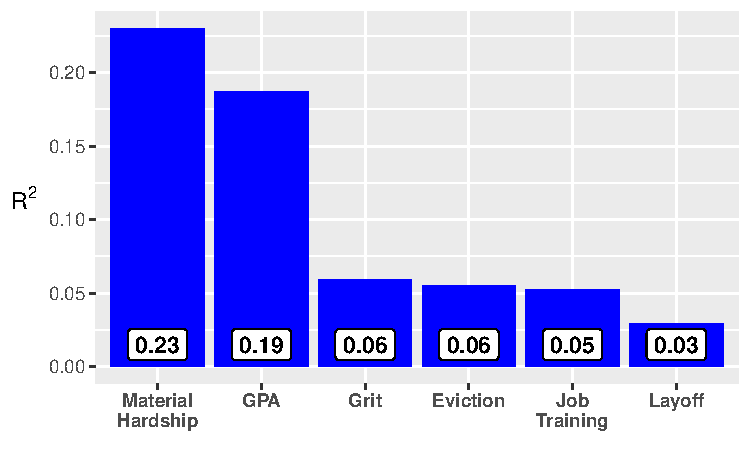
\includegraphics[width=0.95\textwidth]{figures/RSquared_all_ASA.pdf}}
\only<2>{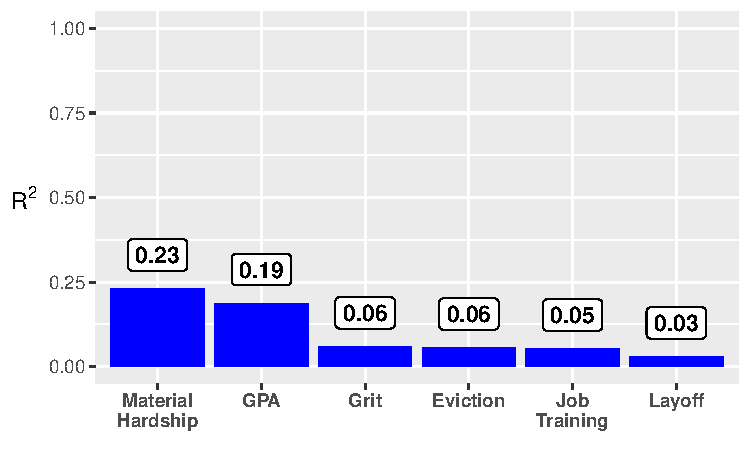
\includegraphics[width=0.95\textwidth]{figures/RSquared_all_ASA_01.pdf}}
\end{center}

\end{frame}
%%%%%%%%%%%%%%%%%%%%%%
\begin{frame}

\begin{center}
\Large{Is this even better than a benchmark model?}
\end{center}

\end{frame}
%%%%%%%%%%%%%%%%%%%
\begin{frame}

\begin{center}
\only<1>{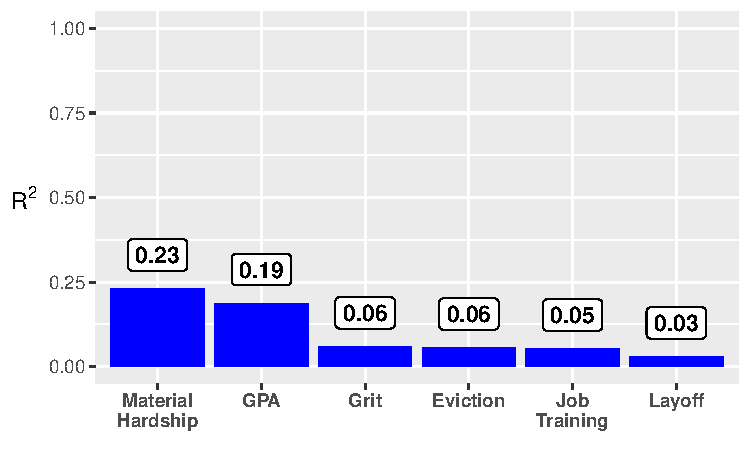
\includegraphics[width=0.95\textwidth]{figures/RSquared_all_ASA_01.pdf}} %
\only<2>{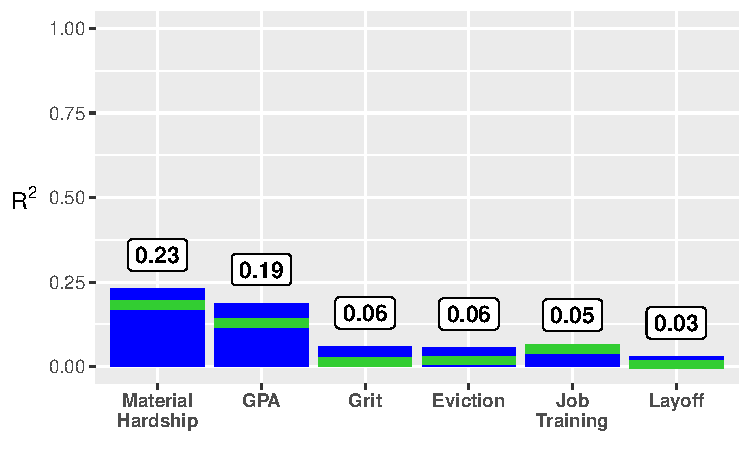
\includegraphics[width=0.95\textwidth]{figures/RSquared_all_ASA_01_benchmark.pdf}} %
\end{center}

\vfill 

\onslide<2>{Green line: 4 variable linear regression model}

\end{frame}
%%%%%%%%%%%%%%%%%%%%%%%%%%%
\begin{frame}

\begin{center}
\only<1>{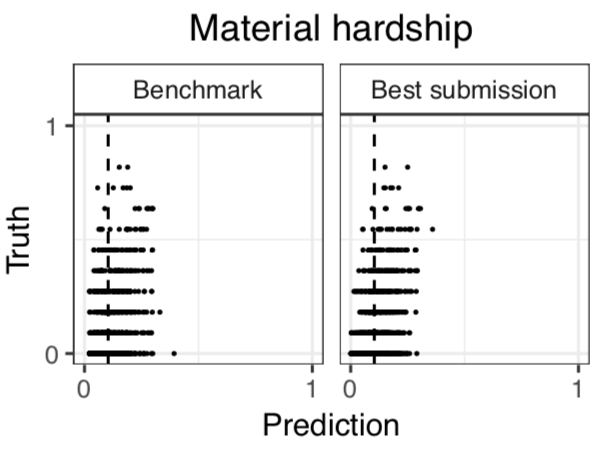
\includegraphics[width=0.95\textwidth]{figures/materialhardship_scatter_best_benchmark}}%
\only<2>{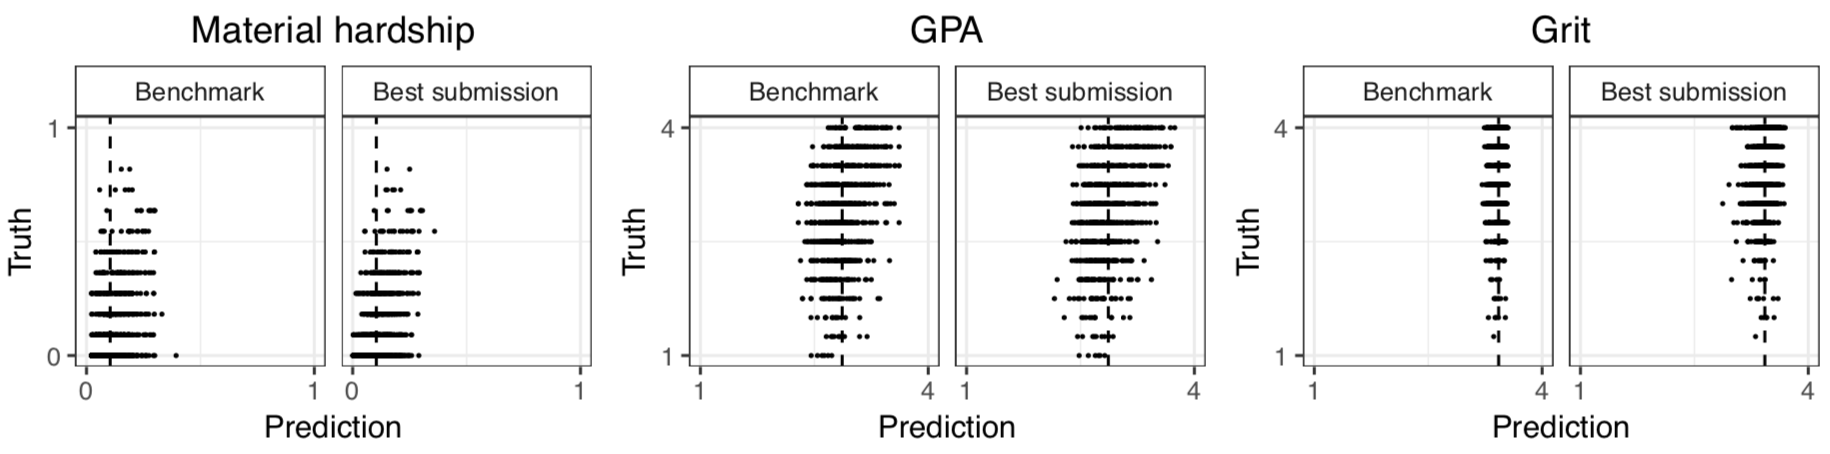
\includegraphics[width=0.95\textwidth]{figures/allcontinuous_scatter_best_benchmark}}%
\end{center}

\end{frame}
%%%%%%%%%%%%%%%%%%%%%%%%%%%
\begin{frame}

\begin{center}
\only<1>{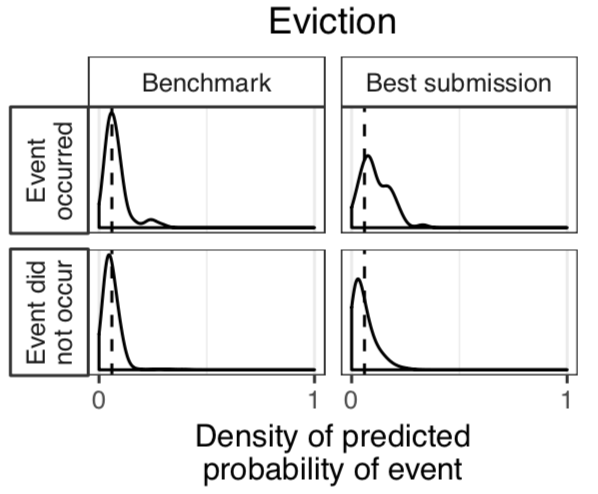
\includegraphics[width=0.95\textwidth]{figures/eviction_density_best_benchmark}}%
\only<2>{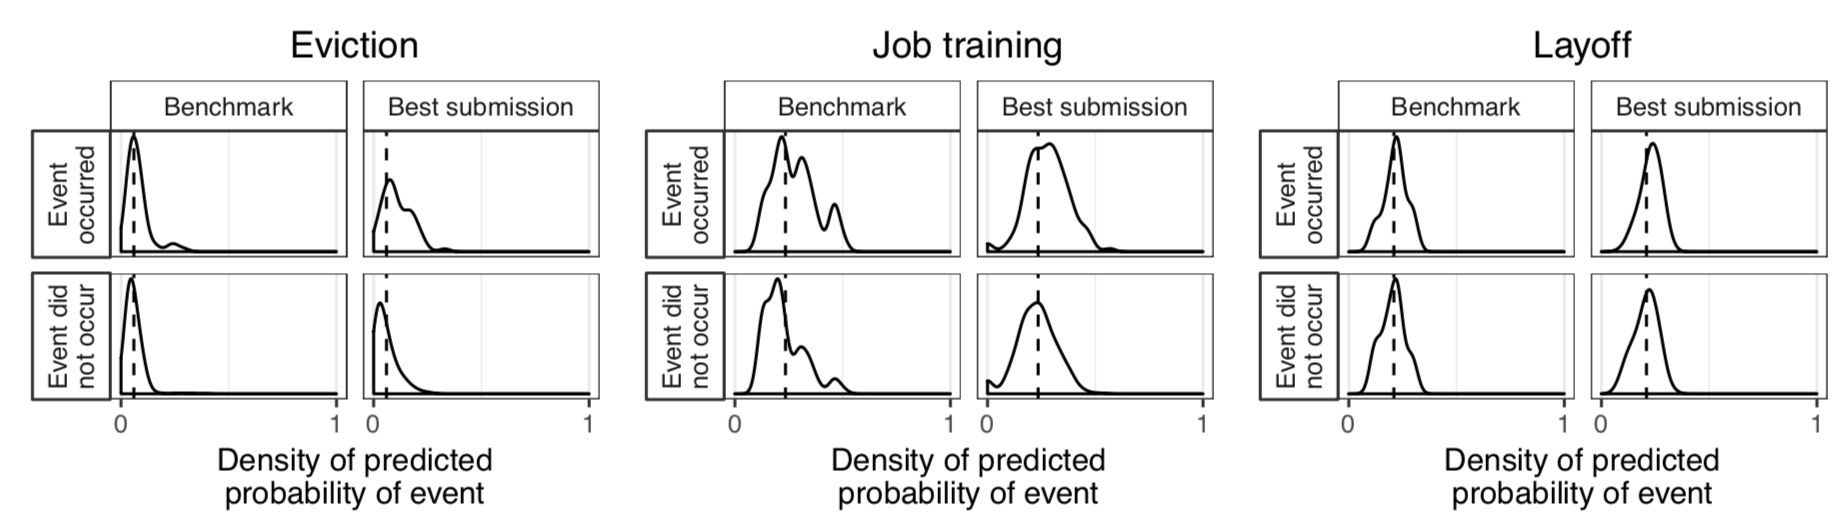
\includegraphics[width=0.95\textwidth]{figures/allbinary_density_best_benchmark}}%
\end{center}

\end{frame}
%%%%%%%%%%%%%%%%%%%%%%%%%%%
\begin{frame}

\begin{center}
\Large{What can we learn looking at the all the predictions?}
\end{center}

\end{frame}
%%%%%%%%%%%%%%%%%%%
\begin{frame}

\begin{center}
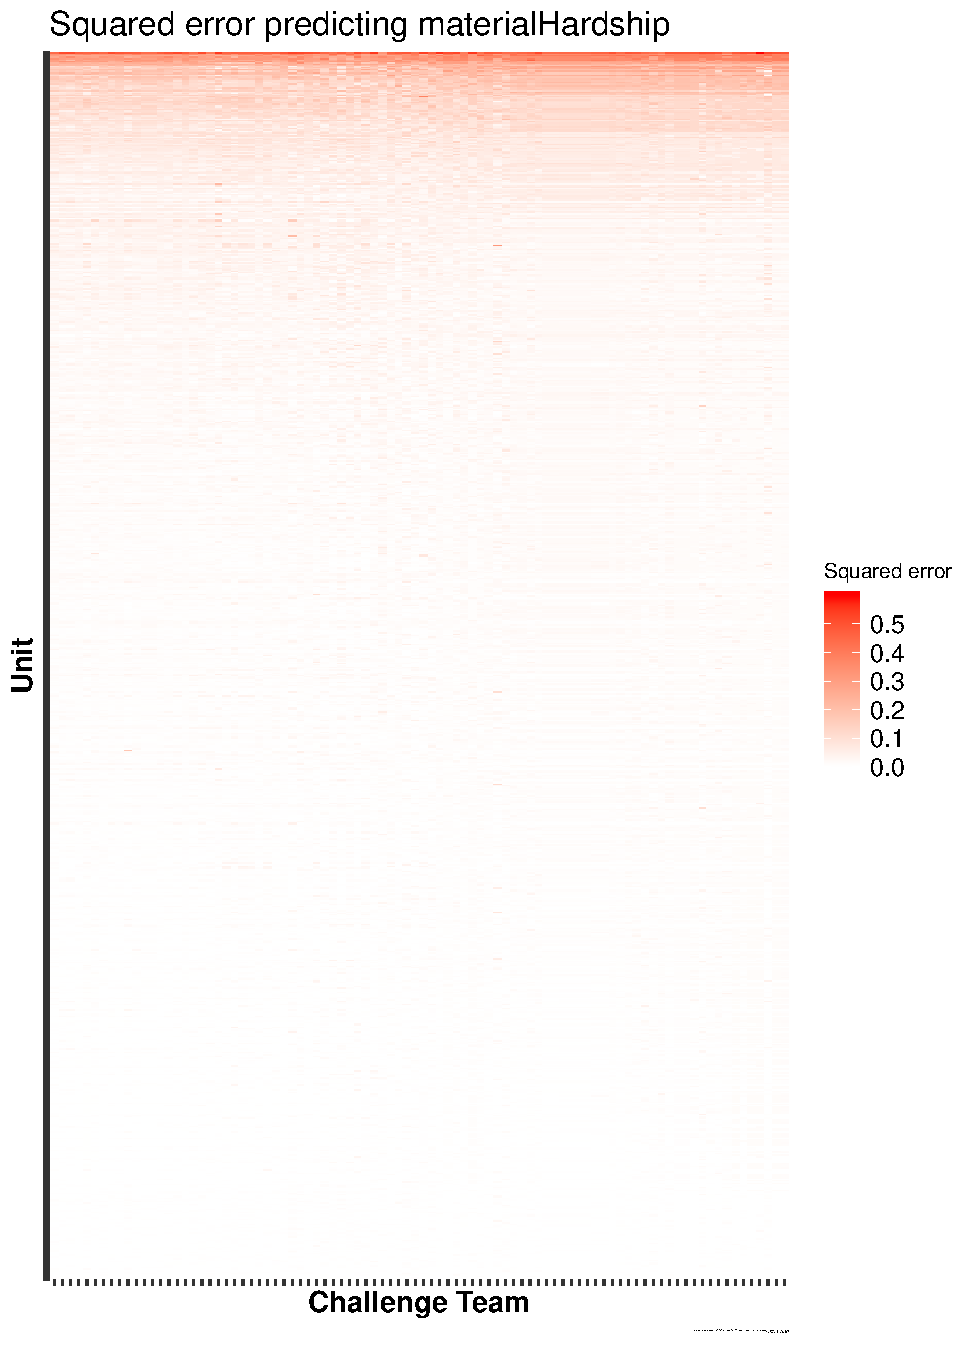
\includegraphics[height=0.90\textheight]{figures/materialHardship_ysort_mse_unit_outcome_xsort_mse_account_outcome.pdf}
\end{center}

\end{frame}
%%%%%%%%%%%%%%%%%%%%%%%%%%
\begin{frame}

\begin{center}
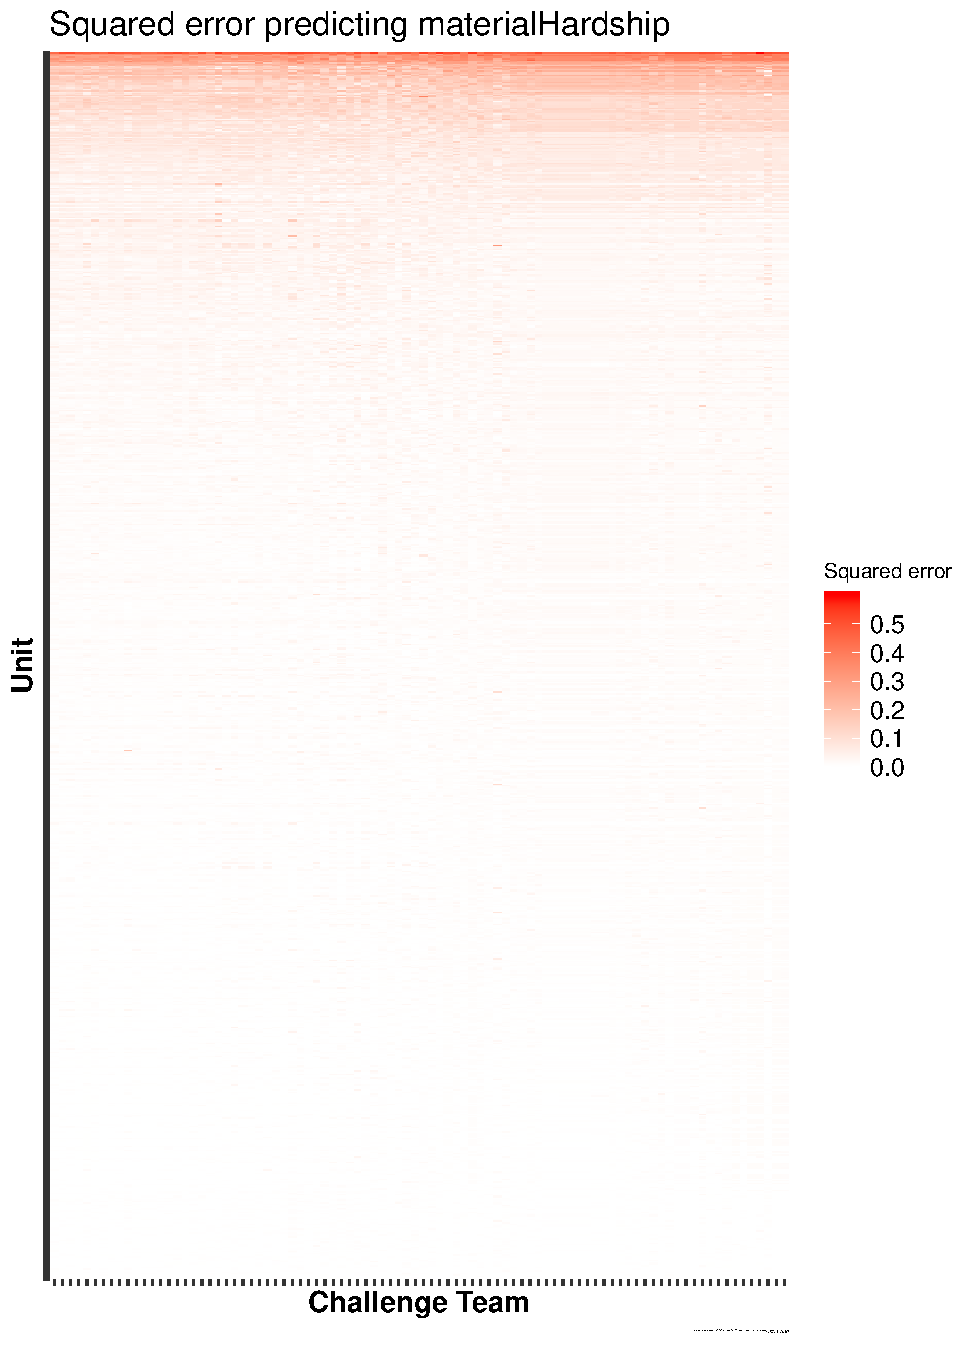
\includegraphics[width=0.30\textheight]{figures/materialHardship_ysort_mse_unit_outcome_xsort_mse_account_outcome.pdf}
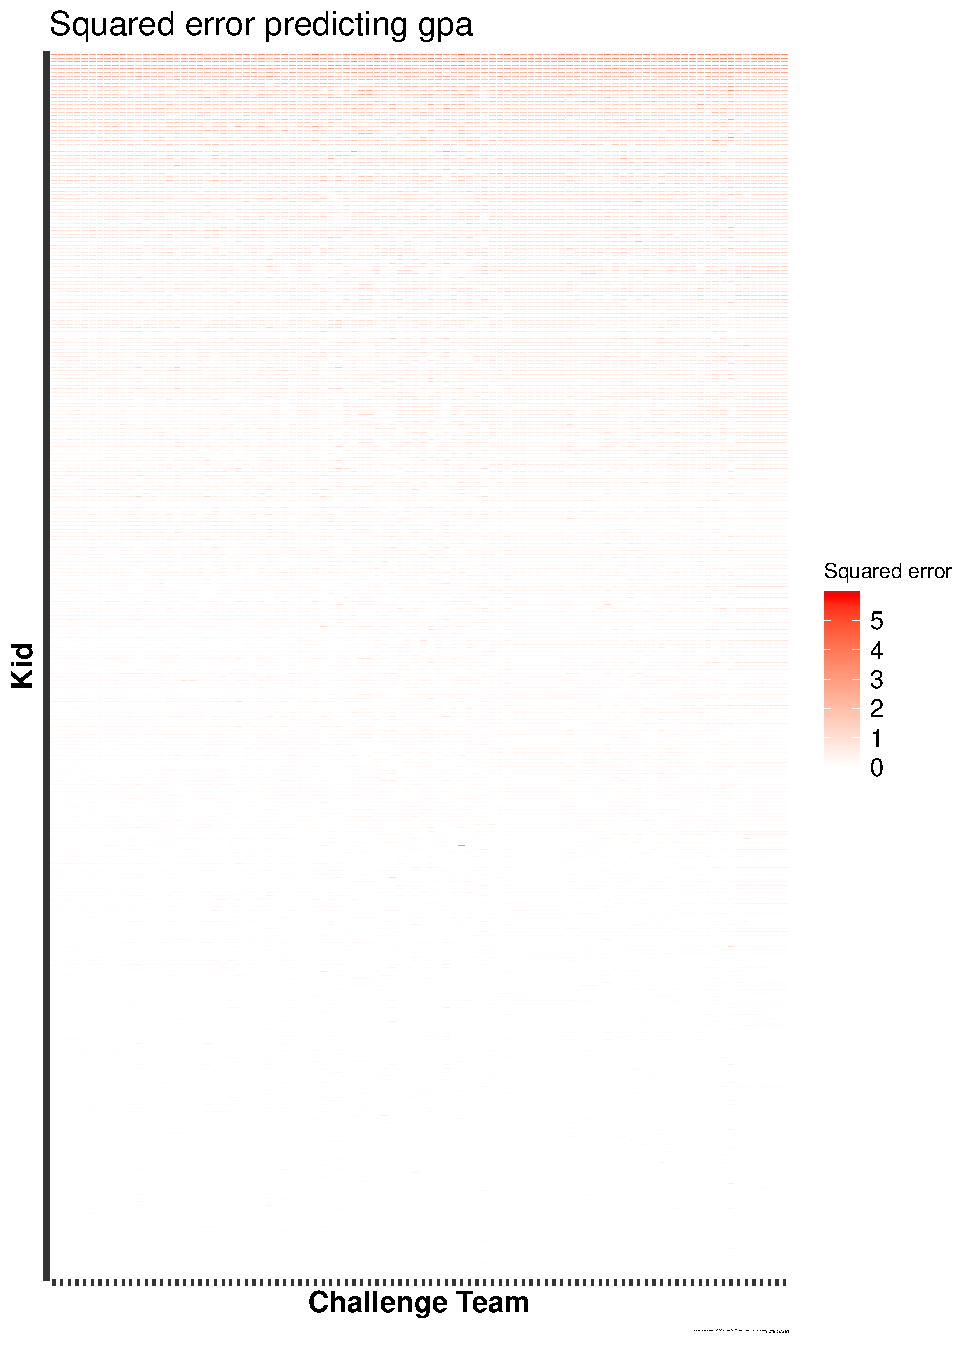
\includegraphics[width=0.30\textheight]{figures/gpa_ysort_mse_unit_outcome_xsort_mse_account_outcome.pdf}
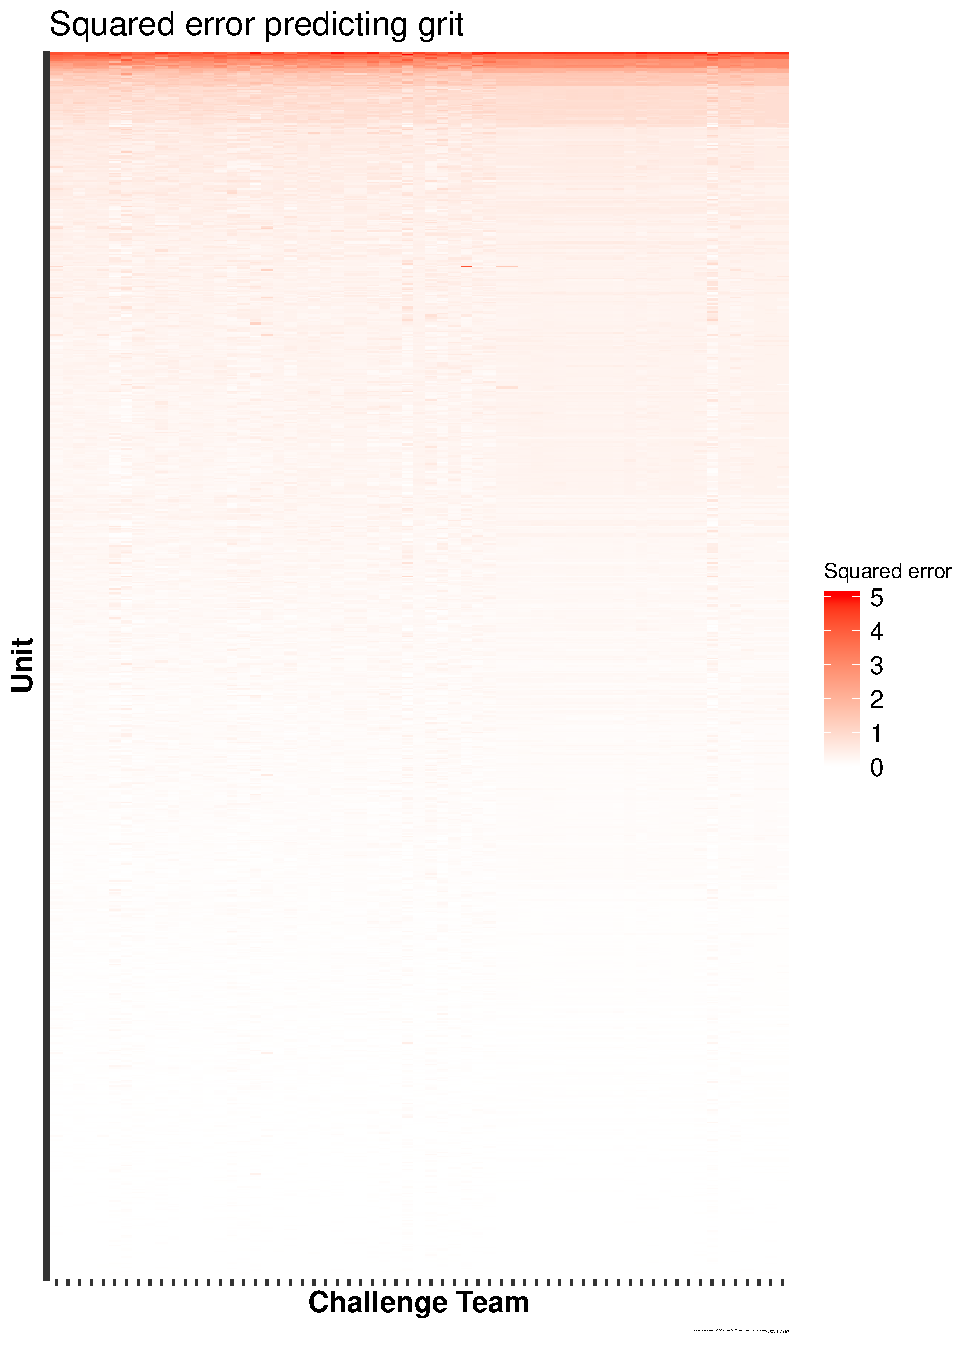
\includegraphics[width=0.30\textheight]{figures/grit_ysort_mse_unit_outcome_xsort_mse_account_outcome.pdf}
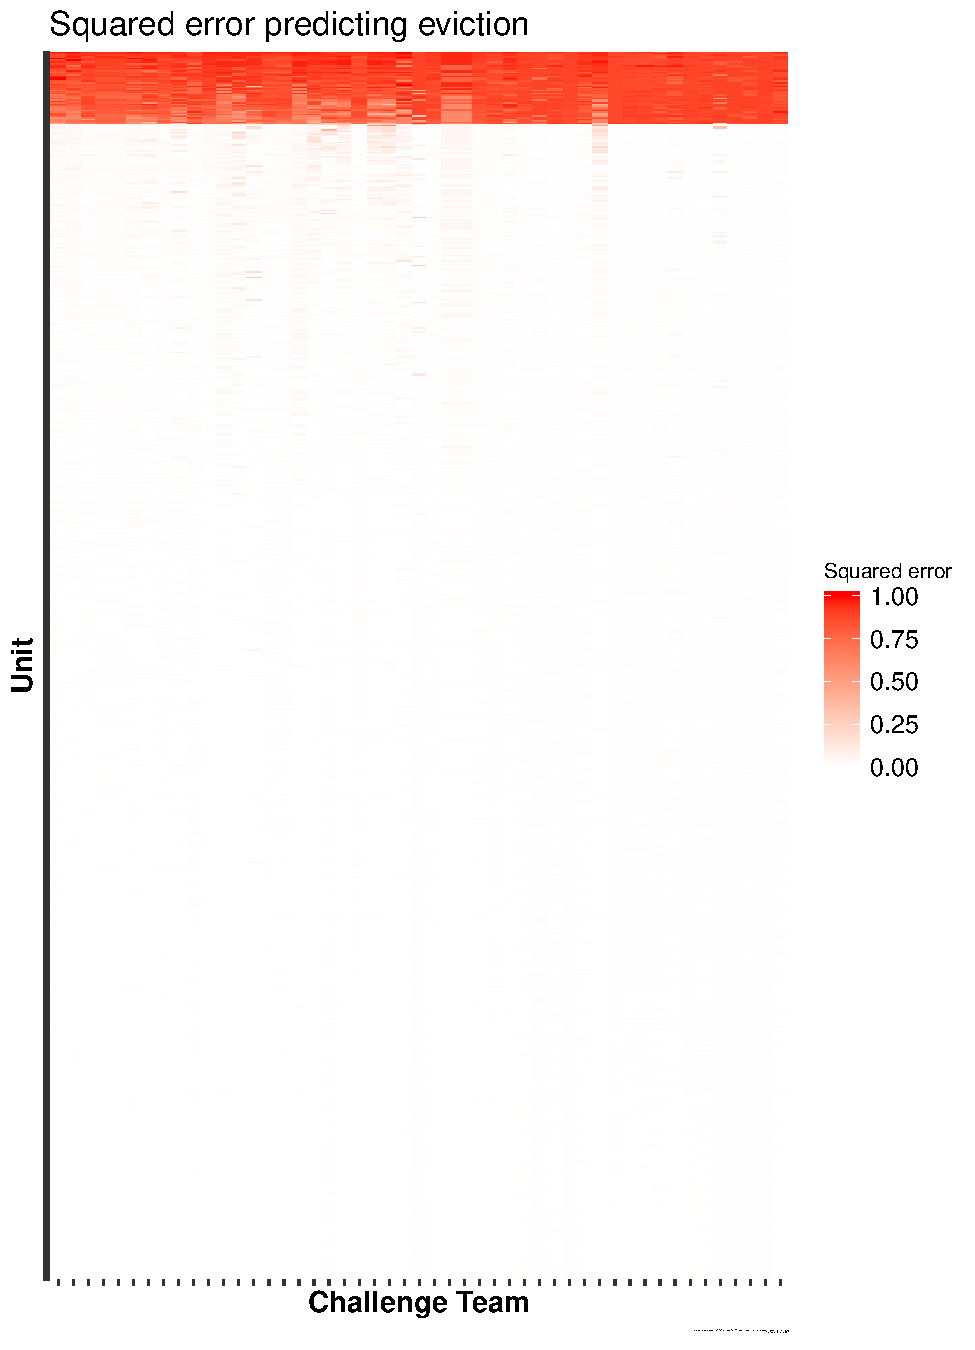
\includegraphics[width=0.30\textheight]{figures/eviction_ysort_mse_unit_outcome_xsort_mse_account_outcome.pdf}
\includegraphics[width=0.30\textheight]{figures/jobtraining_ysort_mse_unit_outcome_xsort_mse_account_outcome.pdf}
\includegraphics[width=0.30\textheight]{figures/layoff_ysort_mse_unit_outcome_xsort_mse_account_outcome.pdf}
\end{center}

\end{frame}
%%%%%%%%%%%%%%%%%%%%%%%%%%
\begin{frame}

\begin{center}
\Large{What do these results mean?}
\end{center}

\end{frame}
%%%%%%%%%%%%%%%%%%%%%%%%%%%%
\begin{frame}

\begin{itemize}
\item Is it possible to get better predictive performance for this data and prediction task?
\pause
\item Why is the unpredictability so high even using modern machine learning methods and what many social scientists would consider to be large and high-quality data?
\end{itemize}

\end{frame}
%%%%%%%%%%%%%%%%%%%%%%%%%%%%
\begin{frame}

Why is the unpredictability so high even using modern machine learning methods and what many social scientists would consider to be large and high-quality data?
\begin{itemize}
\item Not enough cases \pause
\item Measurement error in existing variables (particularly outcomes) \pause
\item Important unmeasured variables 
\end{itemize}

\end{frame}
%%%%%%%%%%%%%%%%%%%%%%%%%%%%%
\begin{frame}

\begin{center}
\Large{How can we learn about important measurement error and unmeasured variables?}
\end{center}

\end{frame}
%%%%%%%%%%%%%%%%%%%%%%%%%%%
\begin{frame}

\begin{center}
\only<1>{\includegraphics[width=\textwidth]{figures/darkmatter_interview_sampling_talk_1}}%
\only<2>{\includegraphics[width=\textwidth]{figures/darkmatter_interview_sampling_talk_2}}%
\only<3>{\includegraphics[width=\textwidth]{figures/darkmatter_interview_sampling_talk_3}}%
\only<4>{\includegraphics[width=\textwidth]{figures/darkmatter_interview_sampling_talk_4}}%
\only<5>{\includegraphics[width=\textwidth]{figures/darkmatter_interview_sampling_talk_5}}%
\only<6>{\includegraphics[width=\textwidth]{figures/darkmatter_interview_sampling_talk_6}}%
\only<7>{\includegraphics[width=\textwidth]{figures/darkmatter_interview_sampling_talk_7}}%
\end{center}

\end{frame}
%%%%%%%%%%%%%%%%%%%%%%%%%%
\begin{frame}

\begin{center}
\includegraphics[width=\textwidth]{figures/kaizen_cycle}
\end{center}

\end{frame}
%%%%%%%%%%%%%%%%%%%%%%%%%%%
\begin{frame}

\begin{center}
\Large{What's next?}
\end{center}

\end{frame}
%%%%%%%%%%%%%%%%%%%%%%%%%%%
\begin{frame}

Next steps:
\begin{itemize}
\item One community paper (including all code and predictions) \pause
\item Special issue of \textit{Socius}
\begin{itemize}
\item 12 submitted manuscripts from Challenge participants (all with accompanying code and computing environment) \pause
\item 3 papers from our group \pause
\begin{itemize}
\item ``Privacy, ethics, and data access: A case study of the Fragile Families Challenge'' by Lundberg, Narayanan, Levy, \& Salganik, \url{https://arxiv.org/abs/1809.00103} \pause
\item ``Improving metadata infrastructure for complex surveys: Insights from the Fragile Families Challenge'' by Kindel, Catena, Hartshorne, Jaeger, Koffman, McLanahan, Phillips, Rouhani, Vinh, \& Salganik, \url{https://osf.io/93ywg/} \pause
\item ``Successes and struggles with computational reproducibility in the Fragile Families Challenge'' by Liu \& Salganik
\end{itemize}
\end{itemize}
\end{itemize}

\end{frame}

%%%%%%%%%%%%%%%%%%%%%%%%%
\begin{frame}

{\Large
\begin{center}
Questions
\end{center}
}

\end{frame}
%%%%%%%%%%%%%%%%%%%%%%%%%%%

\end{document}